\documentclass[12pt,prb,aps,epsf]{article}
\usepackage[utf8]{inputenc}
\usepackage{amsmath}
\usepackage{amsfonts}
\usepackage{amssymb}
\usepackage{graphicx} 
\usepackage{latexsym} 
\usepackage[toc,page]{appendix}
\usepackage{listings}
\usepackage{xcolor}
\usepackage{soul}
\usepackage[T1]{fontenc}
\usepackage{amsthm}
\usepackage{mathtools}
\usepackage{setspace}
\usepackage{array,multirow,makecell}
\usepackage{geometry}
\usepackage{textcomp}
\usepackage{float}
%\usepackage{siunitx}
\usepackage{cancel}
%\usepackage{tikz}
%\usetikzlibrary{calc, shapes, backgrounds, arrows, decorations.pathmorphing, positioning, fit, petri, tikzmark}
\usepackage{here}
\usepackage{titlesec}
%\usepackage{bm}
\usepackage{bbold}
\geometry{hmargin=2cm,vmargin=2cm}

\begin{document}
	
	\title{MP 35 Moteurs}
		\author{Naïmo Davier}
		\date{Agrégation 2018}
	
	\maketitle
	
	\tableofcontents
	
	\pagebreak
	
	\subsection{Introduction}
	Grandeurs d'intérêt : rendement ect...
	
\begin{figure}[h]
	\centering 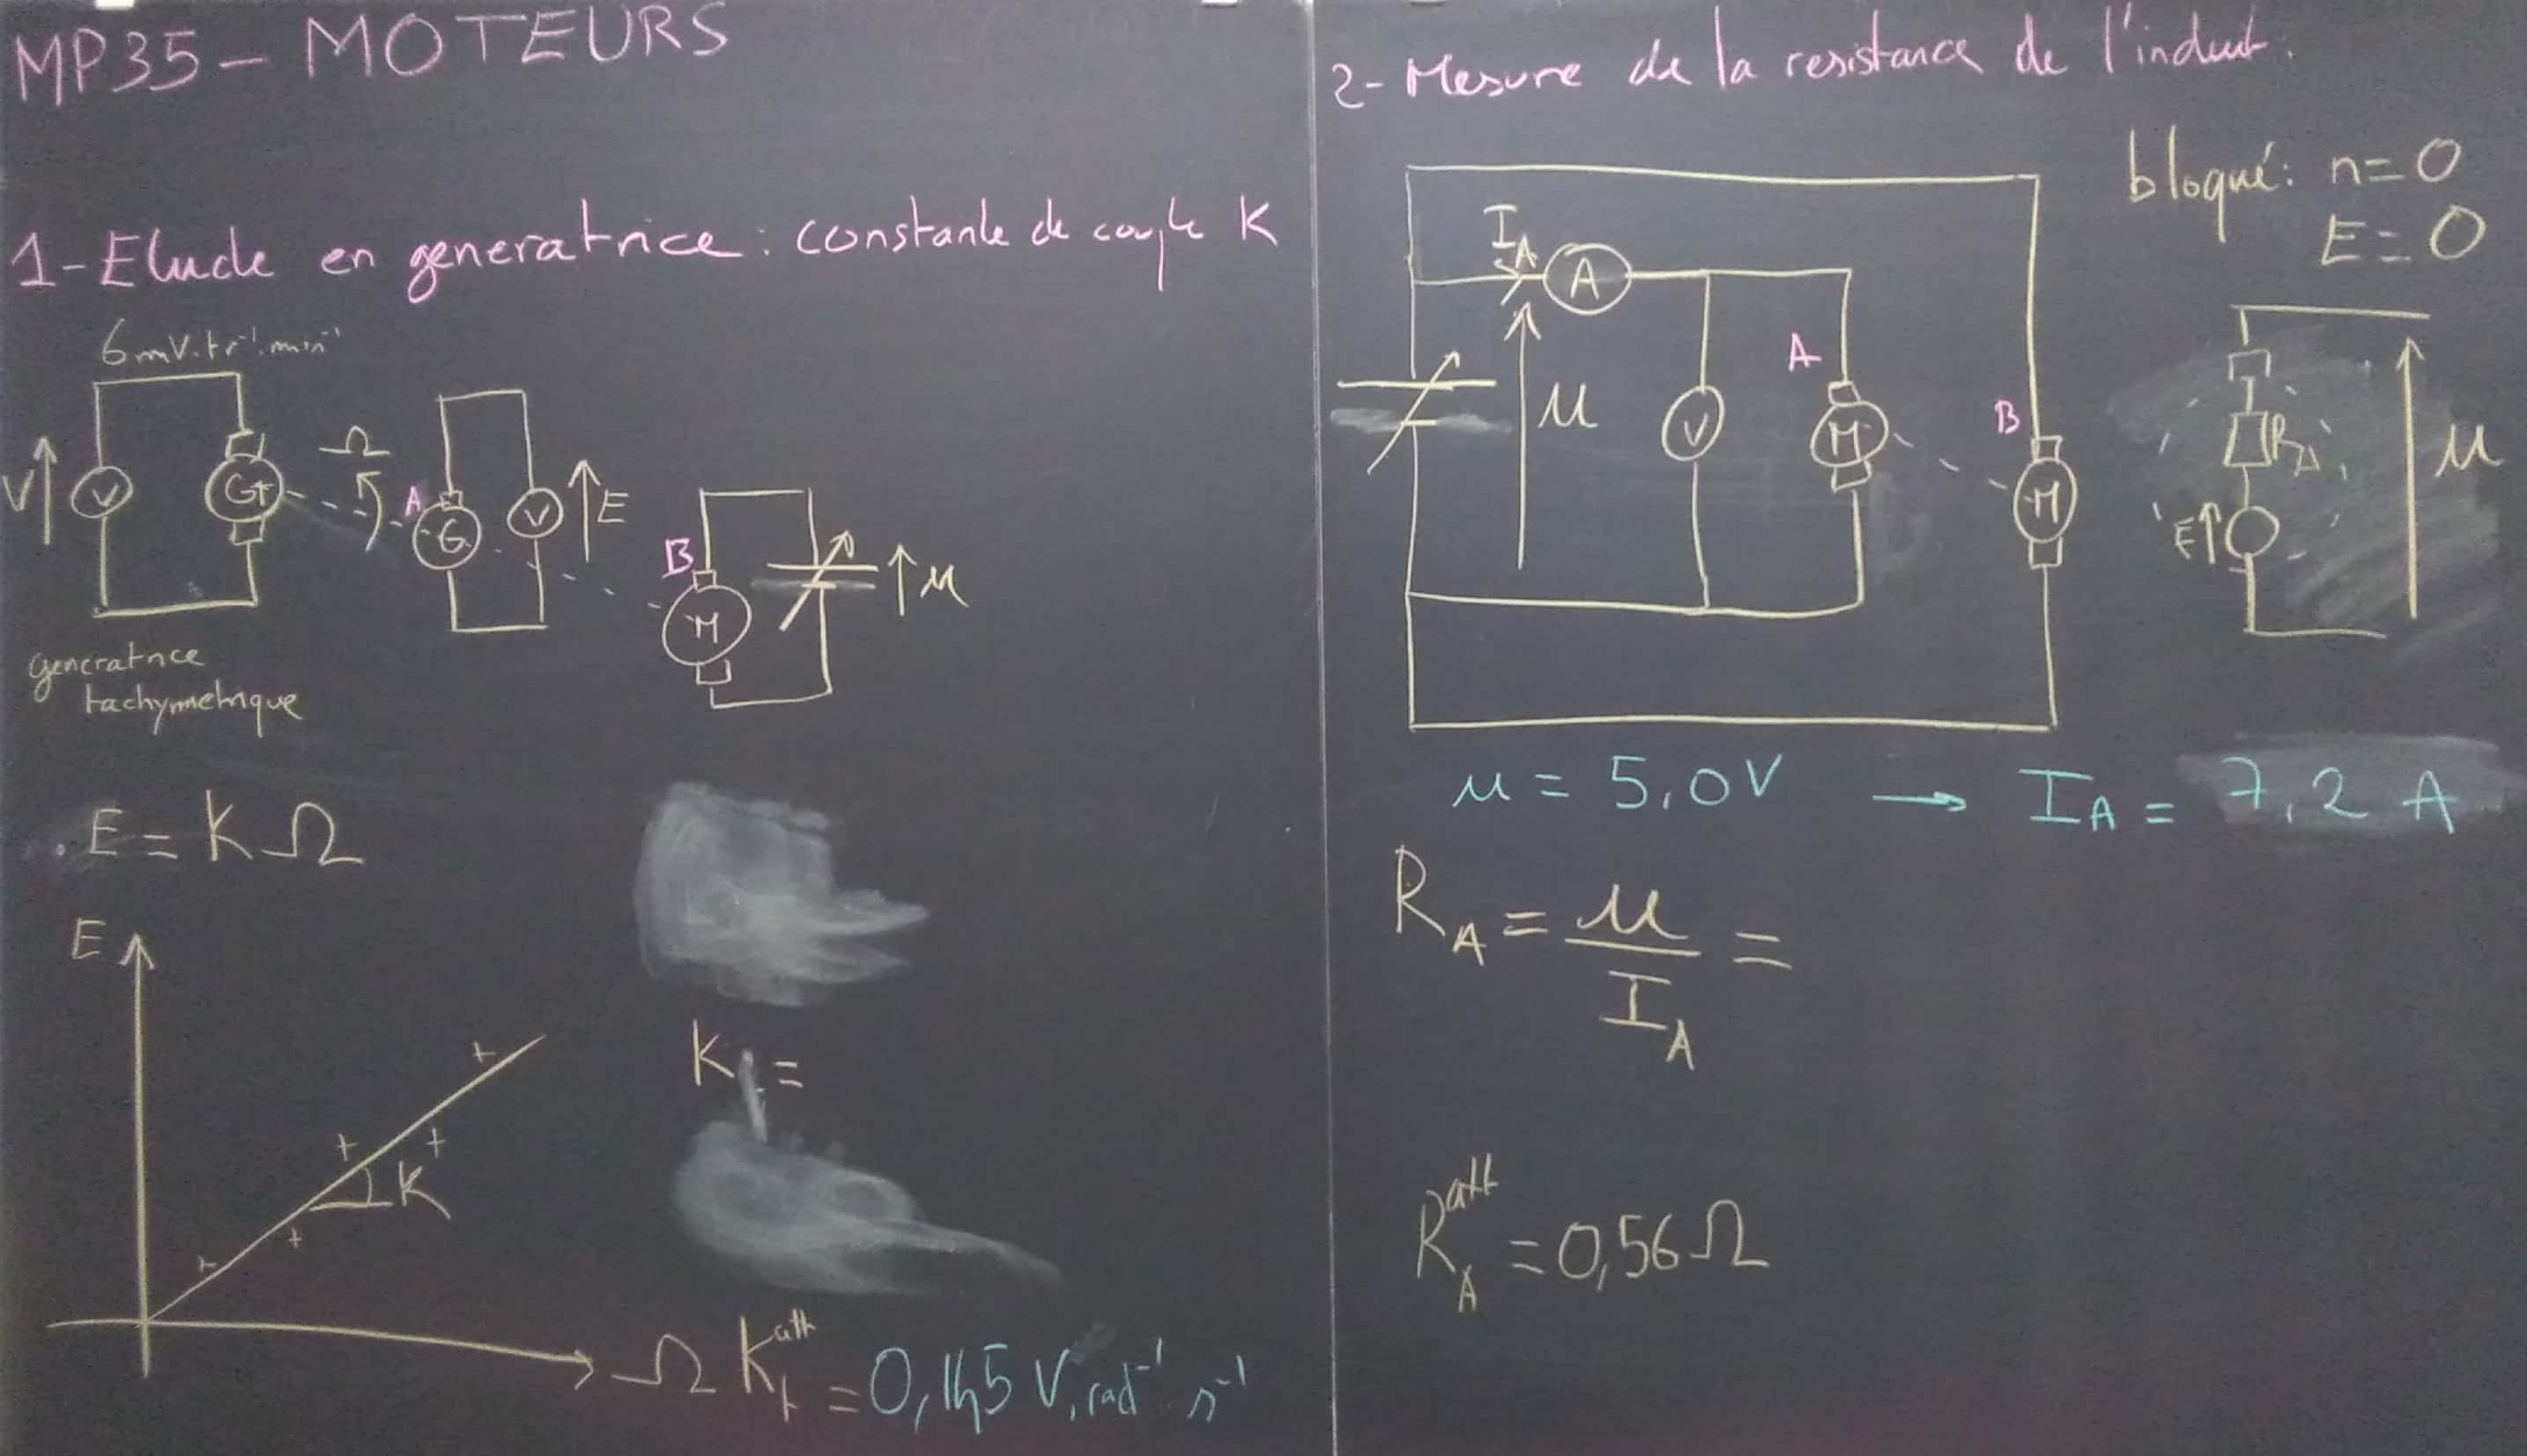
\includegraphics[width=17cm]{t1}
\end{figure}
	
\section{Étude en génératrice : constante de couple K}
On a une sonde tachimétrique pour mesurer la vitesse de rotation $\Omega$. On contrôle l'intensité et la tension fournies au moteur via une alimentation courant tension continue. \\
La constante de couple K est définie comme 
\begin{eqnarray}
E = K\Omega
\end{eqnarray}
On modifie $\Omega$ en jouant sur la tension, on mesure E avec un voltmètre et on trace alors $E=f(\Omega)$, on modélise ensuite par une droite afin de déterminer la constante de couple $K$. On peut ensuite comparer à la valeur donnée dans la doc, soit en $V.m.A^{-1}$ soit en $V.$min/tour.

\section{Mesure de la résistance de l'induit}
On bloque le moteur A en alimentant le moteur B avec la même tension mais de signe opposée, les deux moteurs font donc un bras de fer avec la même force et on a ainsi n=0 et E=0.\\
On mesure alors $V_A$ et $I_A$ avec un voltmètre et on sonde ampèremétrique, pour différentes tension d'alimentation. En traçant $V_A=f(I_A)$ on en déduit la valeur de la résistance de l'induit
\begin{equation}
R_A = \frac{V_A}{I_A}
\end{equation}

\begin{figure}[h]
	\centering 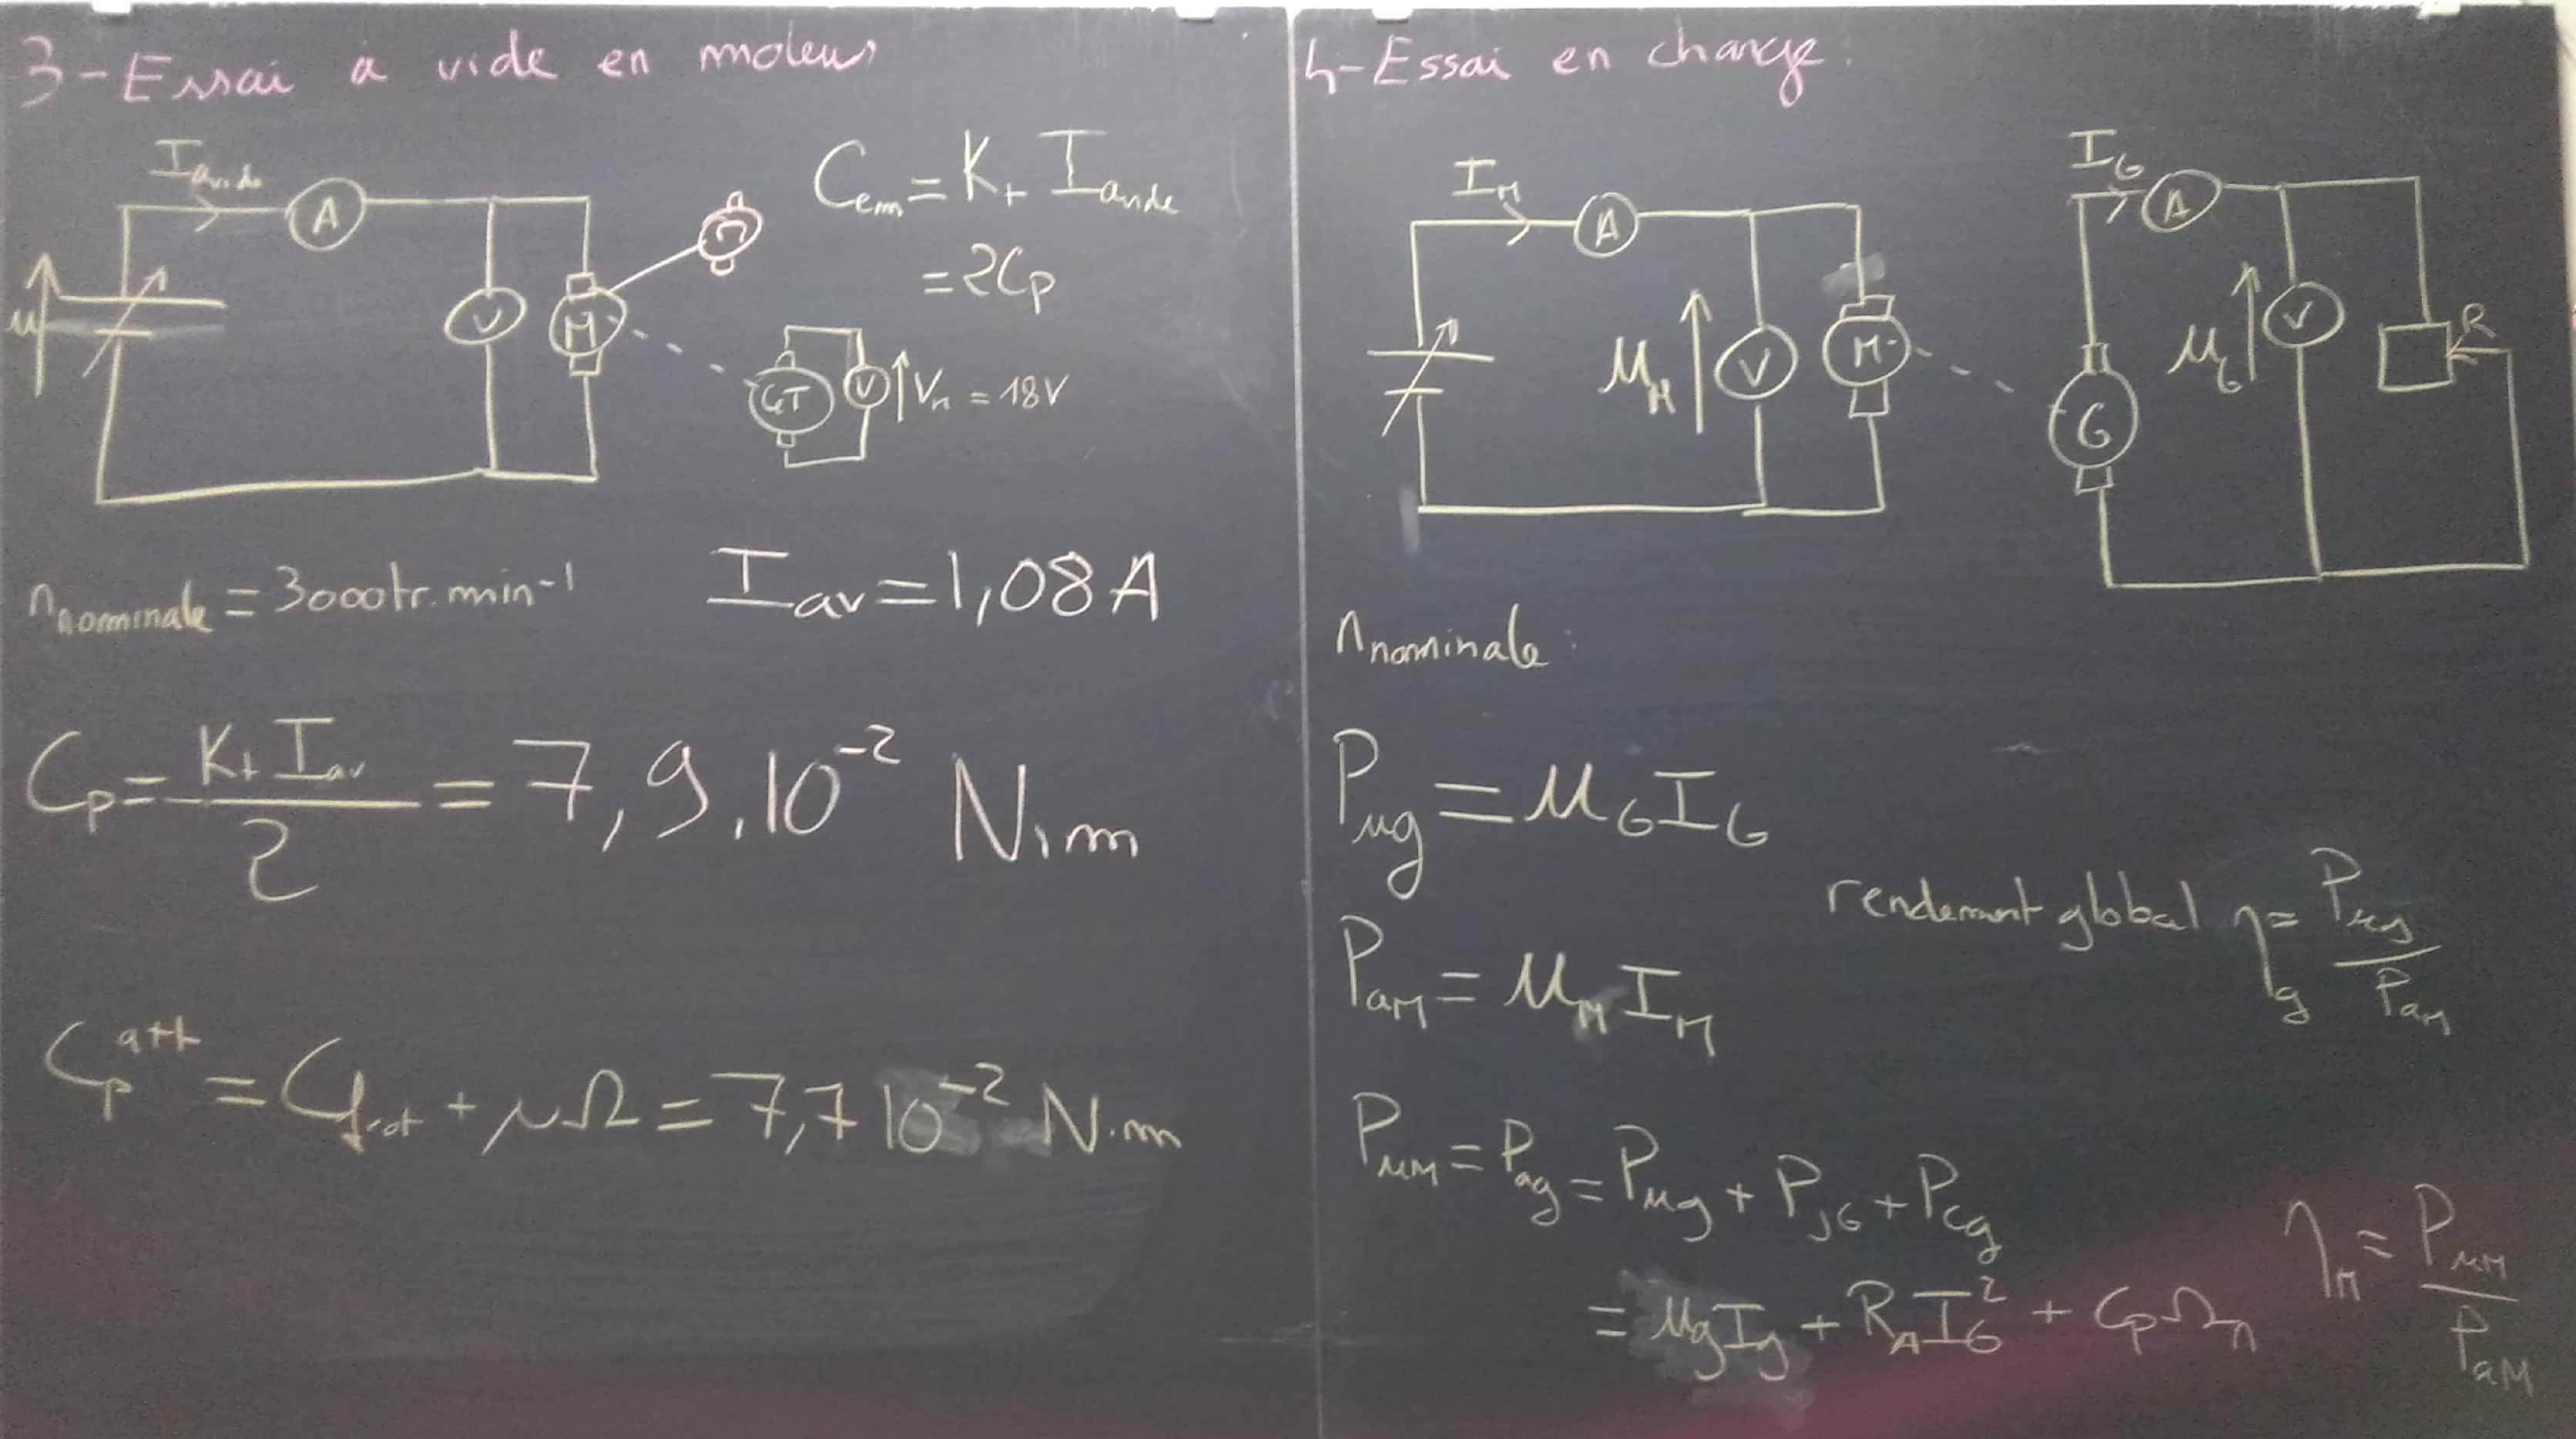
\includegraphics[width=17cm]{t2}
\end{figure}

\section{Essai à vide en moteur}
On fait fonctionner le moteur A à vide (il est toujours relié au moteur B, mais ce dernier n'est pas alimenté). On ajuste la tension d'alimentation afin de se placer à la vitesse de rotation nominale (mesurée à l'aide de la sonde tachimétrique ou d'un voltmètre). On mesure alors 
\begin{equation}
C_{em} = KI_{a\,vide} = 2C_p
\end{equation}
puisque les moteurs étant identiques, et étant donné que l'on entraine le moteur A et B, on mesure deux fois le couple de pertes. On en déduit ainsi une mesure du couple de perte $C_p$.

\section{Essai en charge}
On alimente le moteur A, et on dissipe l'énergie fournie au moteur B (qui est alors en générateur) dans une résistance variable (pouvant supporter de grandes intensité $\simeq$ 6A). On mesure alors $I_A$ et $V_A$ pour le moteur, et $I_G$ et $V_G$ aux bornes de la résistance dissipant l'énergie reçue par le générateur (moteur B). Pour toutes les mesures on ajuste $I_A$ tel que la vitesse de rotation soit nominale.\\

On en déduit un calcul du rendement :
\begin{eqnarray}
P_{uG} = V_GI_G\\
P_{aM} = V_MI_M\\
\mathrm{rendement\;global}\;\; \eta_g = \frac{P_{uG}}{P_{aM}}\\
P_{uM} = P_{aG} &=& P_{uG} + P_{joules\,G} + P_{cG}\\
&=& u_{G}I_G + R_AI_G^2 + C_p\Omega_n\\
\eta_M = \frac{P_{uM}}{P_{aM}}
\end{eqnarray}

On trace alors $\eta_M = f(I_A)$, ce qui permet de déterminer l'intensité nominale, pour laquelle le rendements sera maximum. On trouve un rendement max de l'ordre de 80\%, et on pourra comparer la tension d'alimentation nominale $I_A^n$ avec la valeur fournie dans la doc.

\section*{Questions}
Pour la deuxième manip, pourquoi ne pas simplement enlever l'alimentation et mettre un ohmmètre ?\\
La résistance étant très faible on va mesurer surtout celle des fils et des contacts $\rightarrow$ mesure fausse.\\

Quelle est l'expression générale de $C_{em}$ ? Pourquoi y at'il un couple de perte pour le génératrice si elle n'est pas alimenté ?\\
$C_{em} = C_p + C_u$. Car il y a des frottements mécaniques, et de la perte de fer(on fait tourner le rotor dans le champ généré par des aimants permanents).



\end{document}